\paragraph{Milling}

\begin{figure}[ht]
    \centering
    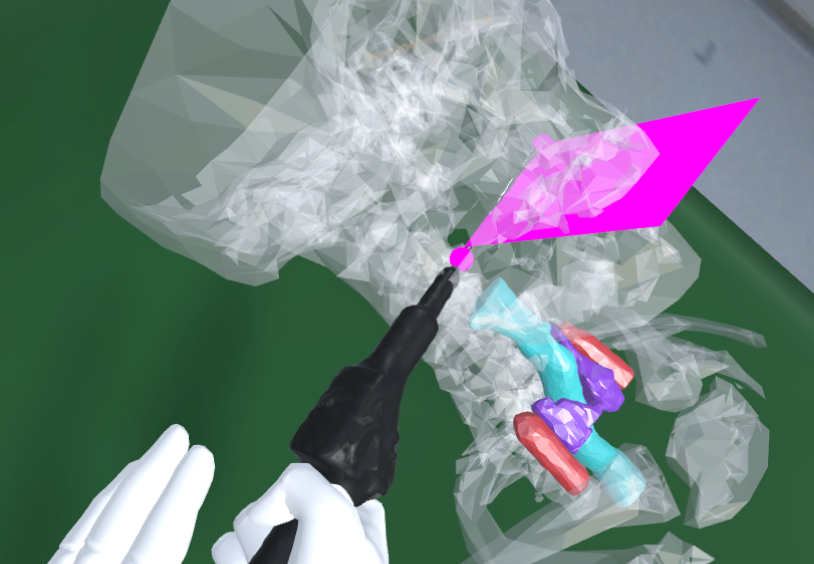
\includegraphics[width=200px]{images/implementation/features/procedures/bonesaw.png}
    \caption{\label{fig::FeaturePiezo}Milling Procedure. Holding down the trigger button will draw little shapes until the button is released.}
\end{figure}

The \textbf{milling} operation is triggered by holding down the trigger button.
While the button is being held down, shapes are being drawn at the tip of the instrument \ref{fig::FeaturePiezo}.
When the button is released, the shapes are combined into a single 3D model and added as a project step.
The procedure which has been performed can this way be reconstructed by "milling" the same 3D space in the virtual operating room.